\documentclass[12pt,spanish,fleqn,openany,letterpaper,pagesize]{scrbook}

\usepackage[ansinew]{inputenc}
\usepackage{url}
\usepackage[spanish]{babel}
\usepackage{fancyhdr}
\usepackage{epsfig}
\usepackage{epic}
\usepackage{eepic}
\usepackage{amsmath}
\usepackage{threeparttable}
\usepackage{amscd}
\usepackage{here}
\usepackage{graphicx}
\usepackage{lscape}
\usepackage{tabularx}
\usepackage{subfigure}
\usepackage{longtable}
\usepackage{xcolor}
\usepackage{algorithm2e}%[linesnumbered,ruled]
\usepackage{fancybox}
\usepackage{tikz}
\usetikzlibrary{babel}
\usetikzlibrary{plotmarks}
\usepackage{pgfplots}
\pgfplotsset{width=7cm,compat=1.8}
\pgfplotsset{%
  colormap={whitered}{color(0cm)=(white);
  color(1cm)=(orange!75!red)}
}
\usepackage{hyperref}
\hypersetup{
    colorlinks,
    citecolor=black,
    filecolor=black,
    linkcolor=black,
    urlcolor=black
}
%\numberwithin{figure}{section}


\usepackage{rotating} %Para rotar texto, objetos y tablas seite. No se ve en DVI solo en PS. Seite 328 Hundebuch
                        %se usa junto con \rotate, \sidewidestable ....


\renewcommand{\theequation}{\thechapter-\arabic{equation}}
\renewcommand{\thefigure}{\textbf{\thechapter-\arabic{figure}}}
\renewcommand{\thetable}{\textbf{\thechapter-\arabic{table}}}


\pagestyle{fancyplain}%\addtolength{\headwidth}{\marginparwidth}
\textheight22.5cm \topmargin0cm \textwidth16.5cm
\oddsidemargin0.5cm \evensidemargin-0.5cm%
\renewcommand{\chaptermark}[1]{\markboth{\thechapter\; #1}{}}
\renewcommand{\sectionmark}[1]{\markright{\thesection\; #1}}
\lhead[\fancyplain{}{\thepage}]{\fancyplain{}{\rightmark}}
\rhead[\fancyplain{}{\leftmark}]{\fancyplain{}{\thepage}}
\fancyfoot{}
\thispagestyle{fancy}%


\addtolength{\headwidth}{0cm}
\unitlength1mm %Define la unidad LE para Figuras
\mathindent0cm %Define la distancia de las formulas al texto,  fleqn las descentra
\marginparwidth0cm
\parindent0cm %Define la distancia de la primera linea de un parrafo a la margen

%Para tablas,  redefine el backschlash en tablas donde se define la posici\'{o}n del texto en las
%casillas (con \centering \raggedright o \raggedleft)
\newcommand{\PreserveBackslash}[1]{\let\temp=\\#1\let\\=\temp}
\let\PBS=\PreserveBackslash

%Espacio entre lineas
\renewcommand{\baselinestretch}{1.1}

%Neuer Befehl f\"{u}r die Tabelle Eigenschaften der Aktivkohlen
\newcommand{\arr}[1]{\raisebox{1.5ex}[0cm][0cm]{#1}}

%Neue Kommandos
\usepackage{Befehle}


%Trennungsliste
\hyphenation {Reaktor-ab-me-ssun-gen Gas-zu-sa-mmen-set-zung
Raum-gesch-win-dig-keit Durch-fluss Stick-stoff-gemisch
Ad-sorp-tions-tem-pe-ra-tur Klein-schmidt
Kohlen-stoff-Mole-kular-siebe Py-rolysat-aus-beu-te
Trans-port-vor-gan-ge}
%\includeonly{Kap1/Kap1,Kap2/Kap2}
\begin{document}
\pagenumbering{roman}
%\newpage
%\setcounter{page}{1}
\begin{center}
\begin{figure}
\centering%

\epsfig{file=HojaTitulo/logoupo_x2.eps,scale=0.3}%
\end{figure}
\begin{figure}
\centering%

\epsfig{file=HojaTitulo/home.eps,scale=.4}%
\end{figure}
\thispagestyle{empty} \vspace*{2.0cm} \textbf{\huge
UPOHOUSE}\\[2.0cm]
\Large\textbf{Alberto Quevedo Rodr\'{i}guez\\Joaqu\'{i}n Roiz Pagador\\Andr\'{e}s Rueda Mar\'{i}n}\\[1.0cm]
\small Universidad Pablo de Olavide\\
Escuela Polit\'{e}cnica Superior\\
Sevilla, Espa\~{n}a\\
2018\\
\end{center}

\newpage{\pagestyle{empty}\cleardoublepage}

\newpage
\begin{center}
\thispagestyle{empty} \vspace*{0cm} \textbf{\huge
UPOCASA}\\[2.0cm]
\Large\textbf{Alberto Quevedo Rodr\'{i}guez\\Joaqu\'{i}n Roiz Pagador\\Andr\'{e}s Rueda Mar\'{i}n}\\[5.0cm]
\textbf{Grado en Ingenieria Inform\'{a}tica en Sistemas de Informaci\'{o}n}\\[4cm]
%Profesor:\\
%Prof. D. Roberto Ruiz S\'{a}nchez\\[4.0cm]
%Dpto. LENGUAJE Y SISTEMAS INFORMÁTICVOS\\
Universidad Pablo de Olavide\\
Escuela Polit\'{e}cnica Superior\
Sevilla, Espa\~{n}a\\
2018\\
\end{center}



\newpage{\pagestyle{empty}\cleardoublepage}

\newpage
\textbf{\LARGE Resumen}
\addcontentsline{toc}{chapter}{\numberline{}Resumen}\\\\
Completa aplicaci\'{o}n funcional y escalable que permite crear y consultar anuncios de compraventa y alquiler de viviendas.\\

\textbf{\small Palabras clave: }\\[2.0cm]



%\textbf{\LARGE Abstract}\\\\
%Complete functional and scalable application based on a management system for clients, machinery and the rental of the same for a fictitious company known as AlkiJardin. This document includes the analysis, design, and implementation requirements for it.\\
%
%\textbf{\small Keywords: AlkiJardin, Engineering, Software, UML, Patterns, Use Cases, Domain Model, Contract, Sequence Diagram, Class Diagram}\\

\newpage{\pagestyle{empty}\cleardoublepage}

\renewcommand{\tablename}{\textbf{Tabla}}
\renewcommand{\figurename}{\textbf{Figura}}
\renewcommand{\listtablename}{Lista de Tablas}
\renewcommand{\listfigurename}{Lista de Figuras}
\renewcommand{\contentsname}{Contenido}


%\newcommand{\clearemptydoublepage}{\newpage{\pagestyle{empty}\cleardoublepage}}
\tableofcontents
%\include{Tab_Simbolos/TabSimbolosMSc}
%\include{Resumen}%\newcommand{\clearemptydoublepage}{\newpage{\pagestyle{empty}\cleardoublepage}}
\pagenumbering{arabic}
%--- INTRO ---
\newpage{\pagestyle{empty}\cleardoublepage}
\newpage{\pagestyle{empty}\cleardoublepage}
\newpage
\vspace*{\fill}
    \begin{center}
      \thispagestyle{empty} \vspace*{0cm} \textbf{\huge
Visi\'{o}n de la Aplicaci\'{o}n}
    \end{center}
    \vspace*{\fill}
\newpage{\pagestyle{empty}\cleardoublepage}
\chapter{Visi\'{o}n de la aplicaci\'{o}n}
\section{Descripci\'{o}n general}


Se desea desarrollar una aplicaci\'{o}n para el sector de la compraventa y alquiler de viviendas, la cual permit\'{a} un acceso r\'{a}pido y p\'{u}blico del listado de anuncios que se hayan publicado. \\

La aplicaci\'{o} deber\'{a} permitir el listado paginado de los anuncios del sistema, as\'{i} como una serie de par\'{a}metros o filtros para personalizar b\'{u}squedas. Del mismo modo, se requerir\'{a} un buscador global en la p\'{a}gina principal que ayude a los usuarios a localizar de forma sencilla y cercana al lenguaje natural un conjunto de anuncios.\\

Para acceder a m\'{a}s funcionalidades, el sistema deber\'{a} permitir que un usuario pueda registrarse e identificarse en el sistema.\\

El sistema debe permitir tambi\'{e}n la gesti\'{o}n de anuncios a los usuarios registrados que los hayan publicado (anunciantes), incluyendo creaci\'{o}n, edici\'{o}n y eliminaci\'{o}n de \'{e}stos.\\

A partir de los anuncios consultados, el usuario podr\'{a} a\~{n}adir comentarios y consultar los existentes, as\'{i} como valorar los propios anuncios de forma sencilla.\\

Para que los usuarios se sientan c\'{o}modos creando los anuncios, se les proporcionar\'{a} una lista de Operaciones y tipos de viviendas asociadas a los anuncios. Tambi\'{e}n se les facilitar\'{a} la selecci\'{o}n de la comunidad aut\'{o}noma, provincia y municipio. La gesti\'{o}n de im\'{a}genes en los anuncios permitir\'{a} al usuario subir varias a la vez, as\'{i} como sustitu\'{i}rlas de manera sencilla.\\

Sobre un anuncio, un usuario registrado interesado podr\'{a} realizar una petici\'{o}n que aparecer\'{a} al anunciante en su zona adecuada para gestionarla, pudiendo aceptarla (rechazando todas las dem\'{a}s asociadas a este anuncio) o rechazarla. Aquel anuncio que estuviera aceptado no deber\'{i}a aparecer en los resultados de b\'{u}squeda. \\ 

Los usuarios registrados podr\'{a}n denunciar a otros usuarios que hayan llevado mal comportamiento en el sistema, peticiones sobre los propios anuncios que crean inadecuadas, anuncios con contenido ofensivo o comentarios no adecuados para la web.

Para todo este sistema se exigir\'{a} tambi\'{e}n la existencia de un rol administrador, el cual permitir\'{a} acceder a una zona especial y reservada conocida como 'dashboard' y en la que se pueda gestionar al completo los usuarios, anuncios, denuncias, tipos de operaciones y tipos de viviendas.

\section{Descripci\'{o}n Detallada}
\subsection{P\'{a}gina Principal}


El usuario visitante podr\'{a} realizar una b\'{u}squeda globalmente en el sistema a trav\'{e}s de un buscador global, as\'{i} como ver de forma ordenada y paginada el listado global de anuncios, en lo posible filtrado seg\'{u}n el tipo de anuncio (en principio compraventa o alquiler) y su tipo de vivienda (en principio casa o piso). Al usuario logado en el sistema se le permitir\'{a} acceder a su perfil desde el navegador principal. Al Administrador, adem\'{a}s, se le proporcionar\'{a} una v\'{i}a de acceso a la zona de gesti\'{o}n.\\

\begin{figure}[h!]
\centering
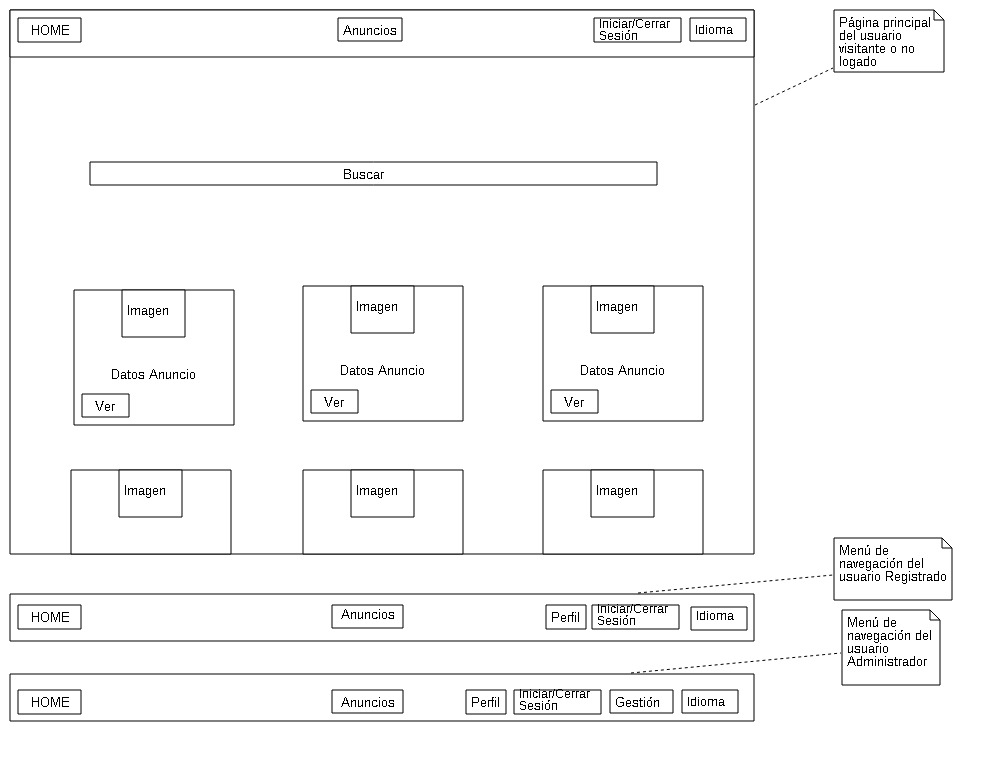
\includegraphics[width=.8\textwidth]{Img/VisionAplicacion/vision_1.jpg}
\end{figure}

Bajo el buscador global aparecer\'{a}n 9 tarjetas adecuadamente situadas con un resumen visual de los \'{u}ltimos 9 anuncios publicados en el sistema, como se plantea en la imagen siguiente:



A trav\'{e}s de estos resultados mostrados se podr\'{a} acceder a los detalles del anuncio en cuesti\'{o}n.\\

En el bot\'{o}n primero del men\'{u} de navegaci\'{o}n superior se mostrar\'{a} alg\'{u}n tipo de imagen o mensaje intuitivo, de forma que el usuario entienda que al hacer click se volver\'{a} a la p\'{a}gina principal.

\subsection{Registro y Login}

Para iniciar sesi\'{o}n en el sistema har\'{a} falta que el usuario est\'{e} registrado. En caso de no estarlo, en la misma secci\'{o}n de acceso se deber\'{a} facilitar al usuario un formulario de inscripci\'{o}n, m\'{i}nimamente con los datos nombre, apellidos, email, tel\'{e}fono, usuario (o username)y contrase\~{n}a. Todos estos datos ser\'{a}n obligatorios. 


\begin{figure}[h!]
\centering
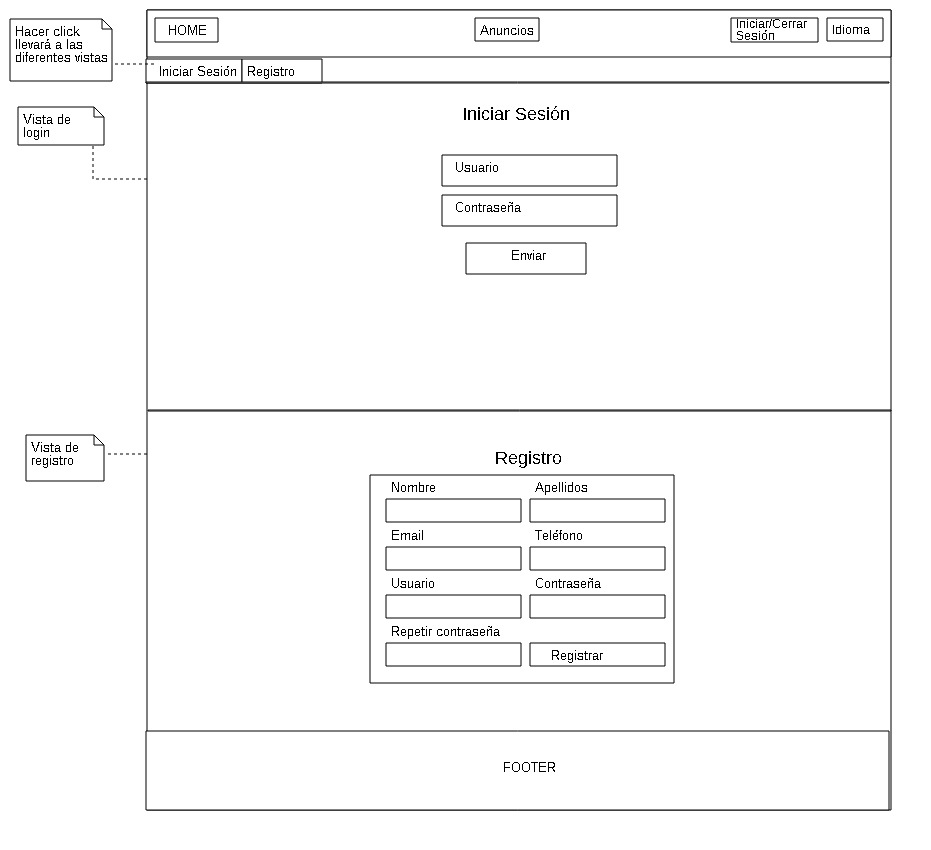
\includegraphics[width=.9\textwidth]{Img/VisionAplicacion/vision_2.jpg}
\end{figure}


\subsection{Listado de anuncios}
El usuario invitado (as\'{i} como registrado o administrador) podr\'{a} listar el conjunto total de anuncios paginados correctamente y con la posibilidad de filtrar por tipo de operaci\'{o}n (como alquiler o compra) y tipo de vivienda (piso o casa). No se deber\'{a}n cargar muchos resultados por p\'{a}gina. De los anuncios se requiere mostrar una miniatura de alguna de sus im\'{a}genes, en caso de tener, un t\'{i}tulo asociado al tipo de vivienda y su zona, su precio, habitaciones, metros cuadrados y localizaci\'{o}n. Tambi\'{e}n su descripci\'{o}n limitada a unas pocas palabras y cu\'{a}ndo se public\'{o}. A trav\'{e}s de estos resultados mostrados se podr\'{a} acceder a los detalles del anuncio en cuesti\'{o}n.

Esta misma vista ser\'{a} utilizada para listar los anuncios de un usuario en particular.


\begin{figure}[h!]
\centering
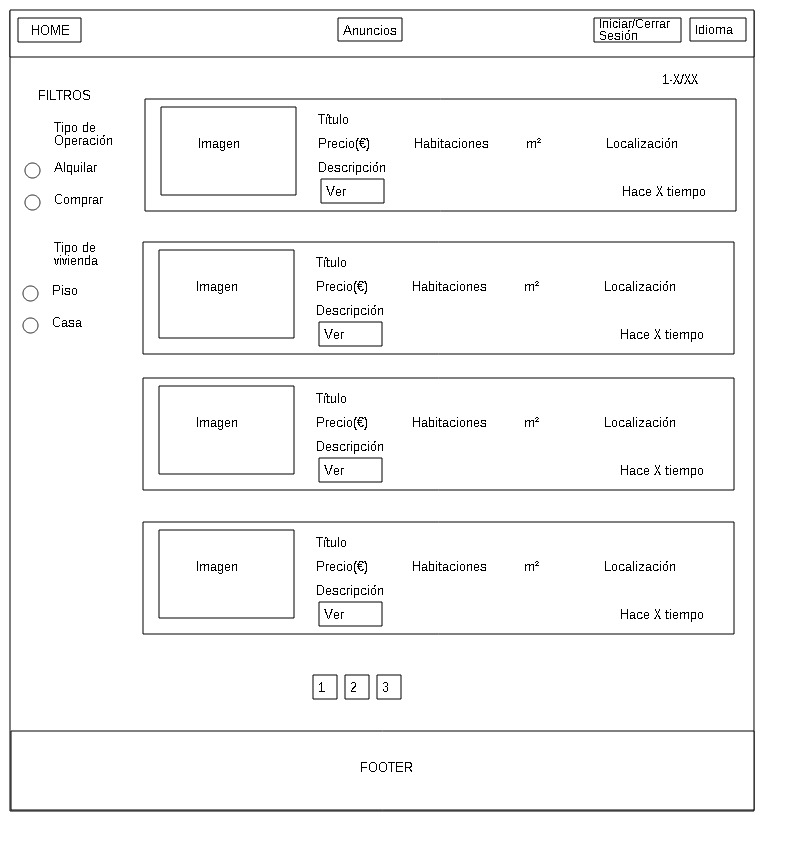
\includegraphics[width=.6\textwidth]{Img/VisionAplicacion/vision_3.jpg}
\end{figure}

En caso de haber utilizado el buscador global y haber pulsado intro al escribir se mostrar\'{a} una p\'{a}gina con contenido similar al listado de anuncios, pero sin posibilidad de filtrar. El aspecto de las tarjetas mostradas ser\'{a} el mismo que las listadas en la p\'{a}gina principal. Se paginar\'{a} este resultado.

\begin{figure}[h!]
\centering
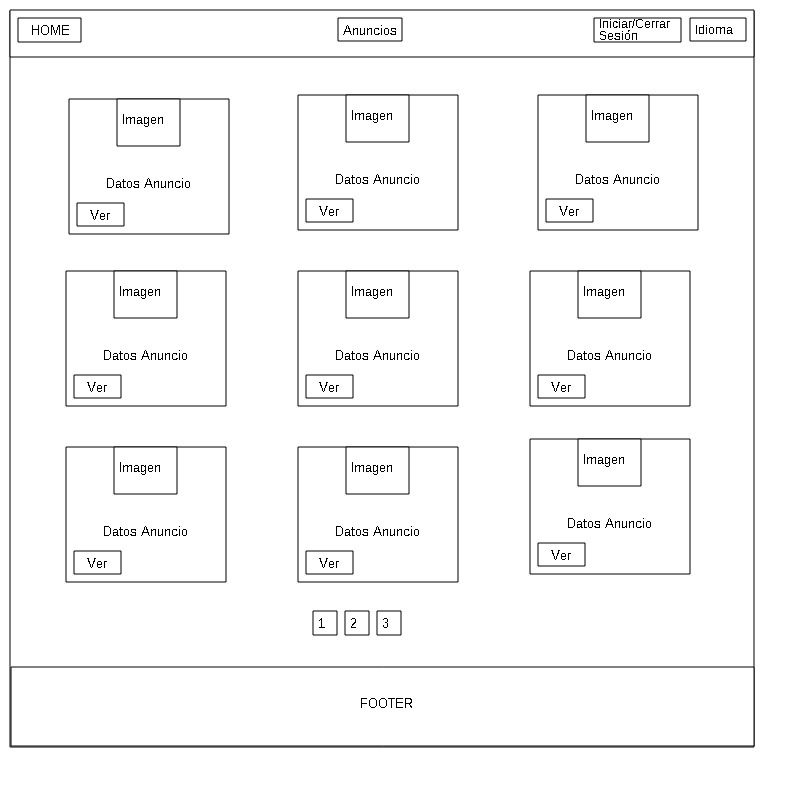
\includegraphics[width=1\textwidth]{Img/VisionAplicacion/vision_10.jpg}
\end{figure}


\subsection{Perfil de Usuario}
A trav\'{e}s del men\'{u} principal, cada usuario podr\'{a} consultar su propio perfil, donde podr\'{a} en contrar un formulario con sus datos para editarlos, menos correo electr\'{o}nico y nombre de usuario.\\

Tambi\'{e}n existir\'{a} un panel de informaci\'{o}n con la cantidad de anuncios publicados por el usuario (y a trav\'{e}s del cual se podr\'{a} llegar al listado mostrado en el punto anterior) y comentarios.\\

Paginando una tarjeta junto a los datos del perfil del usuario, se mostrar\'{a} una peque\~{n}a tabla con el listado de solicitudes que el usuario haya recibido en sus anuncios. Se mostrar\'{a} el usuario asociado a la solicitud, contacto y el contenido escrito por el mismo para ponerse en contacto. Se le facilitar\'{a} al usuario registrado la posibilidad de denunciar dicha solicitud, aceptarla y rechazarla.

\begin{figure}[h!]
\centering
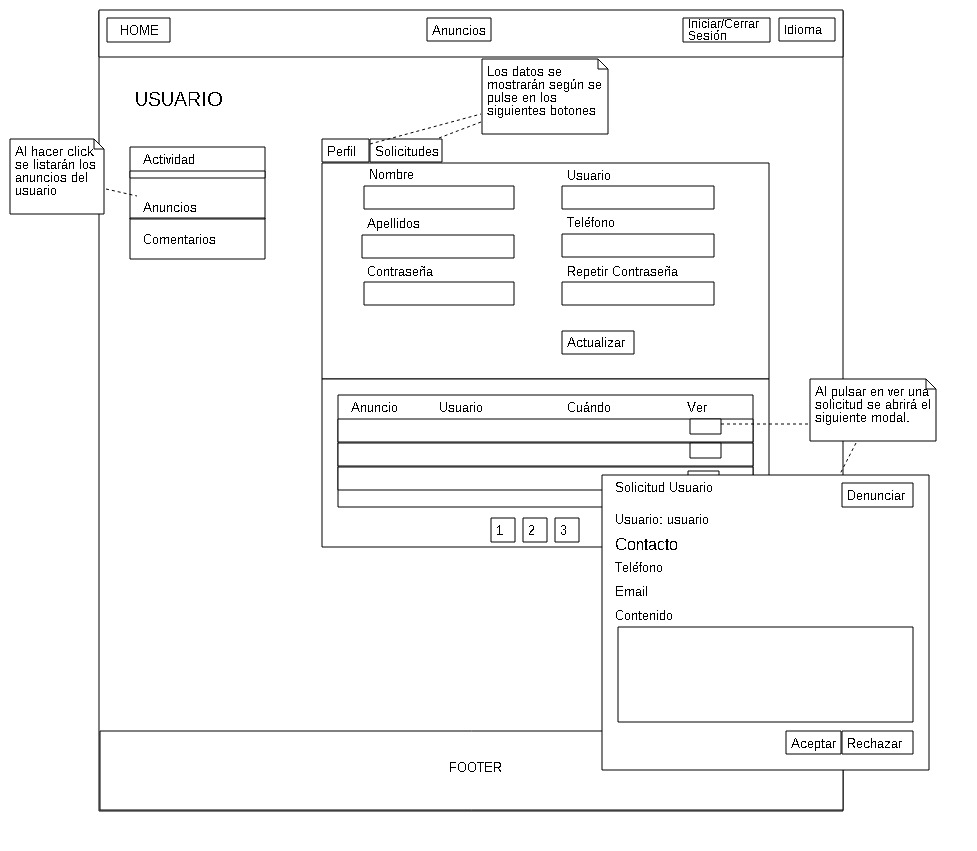
\includegraphics[width=1\textwidth]{Img/VisionAplicacion/vision_4.jpg}
\end{figure}

Por otro lado, si se consultara al usuario asociado a la solicitud o cualquier otro usuario, se mostrar\'{i}a la siguiente vista, donde s\'{o}lamente se muestran sus datos, sin posibilidad de editar. El usuario administrador dispondr\'{a} de dos botones extra para bloquear o eliminar al usuario.\\

\begin{figure}[h!]
\centering
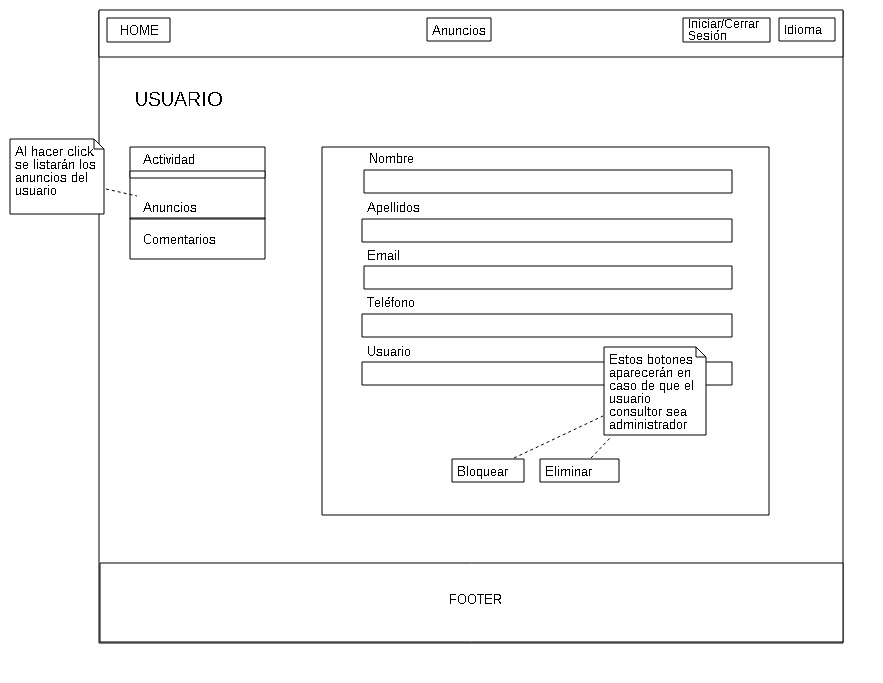
\includegraphics[width=1\textwidth]{Img/VisionAplicacion/vision_5.jpg}
\end{figure}

\pagebreak

\subsection{Anuncios}

Al consultar un anuncio desde cualquier vista se observar\'{a}n todos los detalles asociados al mismo: 
tipo de vivienda, tipo de operaci\'{o}n, precio n\'{u}mero de habitaciones, metros cuadrados, n\'{u}mero de ba\~{n}os, descripci\'{o}n, comunidad aut\'{o}noma, provinciay localidad.\\

Tambi\'{e}n se mostrar\'{a} una galer\'{i}a de fotos, donde se permitir\'{a} ampliar las im\'{a}genes haciendo click en ellas.\\

Debajo de \'{e}stas aparecer\'{a} un peque\~{n}o formulario para crear un comentario, en caso de que el usuario haya iniciado sesi\'{o}n, seguido de un listado de comentarios previamente existentes que se podr\'{a} consultar sin sesi\'{o}n activa. En caso de estar logado en el sistema se podr\'{a} denunciar un comentario si se cree conveniente.\\

\begin{figure}[h!]
\centering
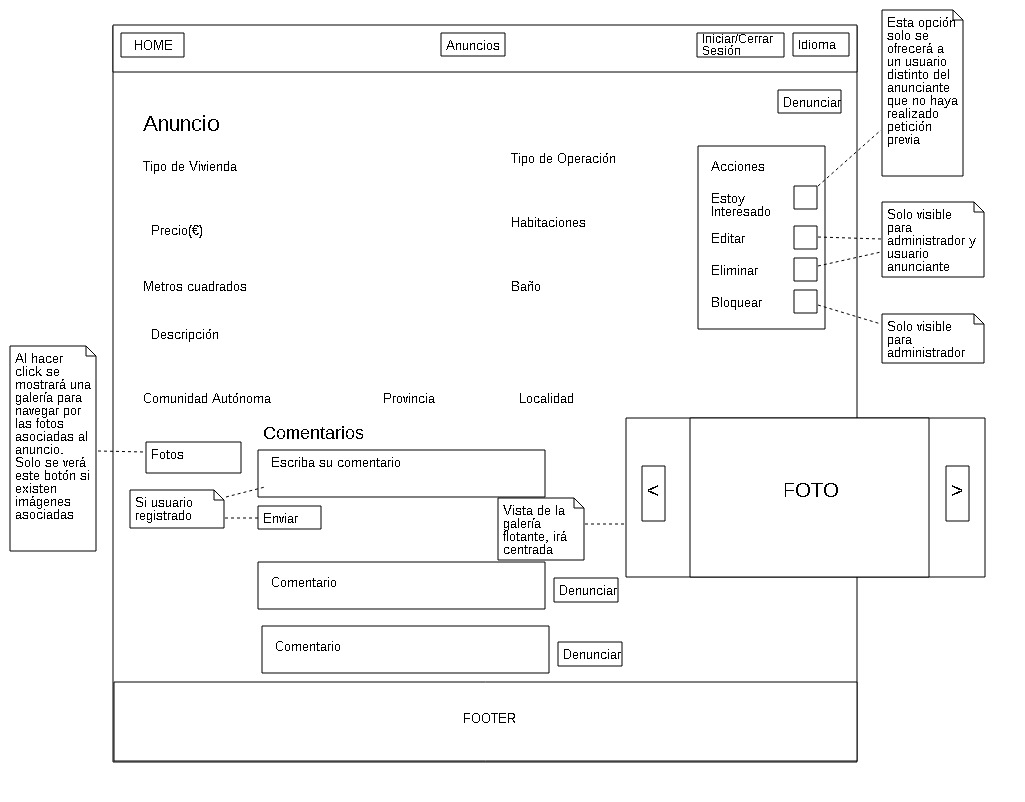
\includegraphics[width=1\textwidth]{Img/VisionAplicacion/vision_6.jpg}
\end{figure}

A la derecha de los datos del anuncio se ver\'{a} un peque\~{n}o panel que muestre las acciones disponibles sobre el anuncio, como realizar una petici\'{o}n (en caso de no ser el propio anunciante o existir una petici\'{o}n previa del usuario sobre ese mismo anuncio), edici\'{o}n y eliminaci\'{o}n (si administrador o usuario anunciante) o bloqueo del anuncio (si usuario administrador). \\

Encima de este panel se ofrecer\'{a} un bot\'{o}n para denunciar el anuncio.



\subsection{Creaci\'{o}n de anuncios}



Los usuarios que quieran publicar un anuncio deber\'{a}n registrarse y logarse en el sistema. 
En el alta del anuncio el usuario decidir\'{a} si quiere ofrecer una venta o alquiler, su precio, metros cuadrados, descripci\'{o}n y aportar fotos. \\

Del mismo modo, se proveer\'{a} a los usuarios de la posibilidad de modificar y retirar sus anuncios. 


\begin{figure}[h!]
\centering
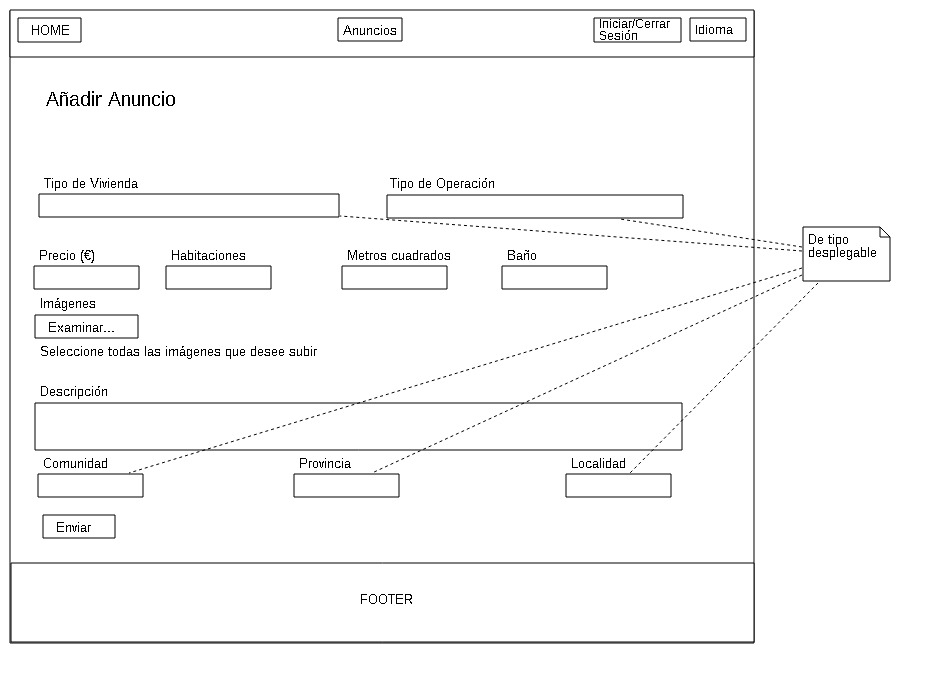
\includegraphics[width=1.1\textwidth]{Img/VisionAplicacion/vision_7.jpg}
\end{figure}


\subsection{Dashboard}
\subsubsection{Usuarios}
Del usuario administrador se espera que se pueda realizar las mismas funciones que un usuario registrado, aparte de sus tareas de administraci\'{o}n, como puedan ser la gesti\'{o}n de usuarios, anuncios y comentarios, de forma que si alg\'{u}n comentario o anuncio fuera ofensivo, \'{e}ste lo borrar\'{i}a y bloquear\'{i}a al usuario, o si existiera alguna denuncia asociada a alguno de estos y fuera debidamente revisada y verificada, se podr\'{i}a aceptar y bloquear autom\'{a}ticamente o, por el contrario, rechazar.

\begin{figure}[h!]
\centering
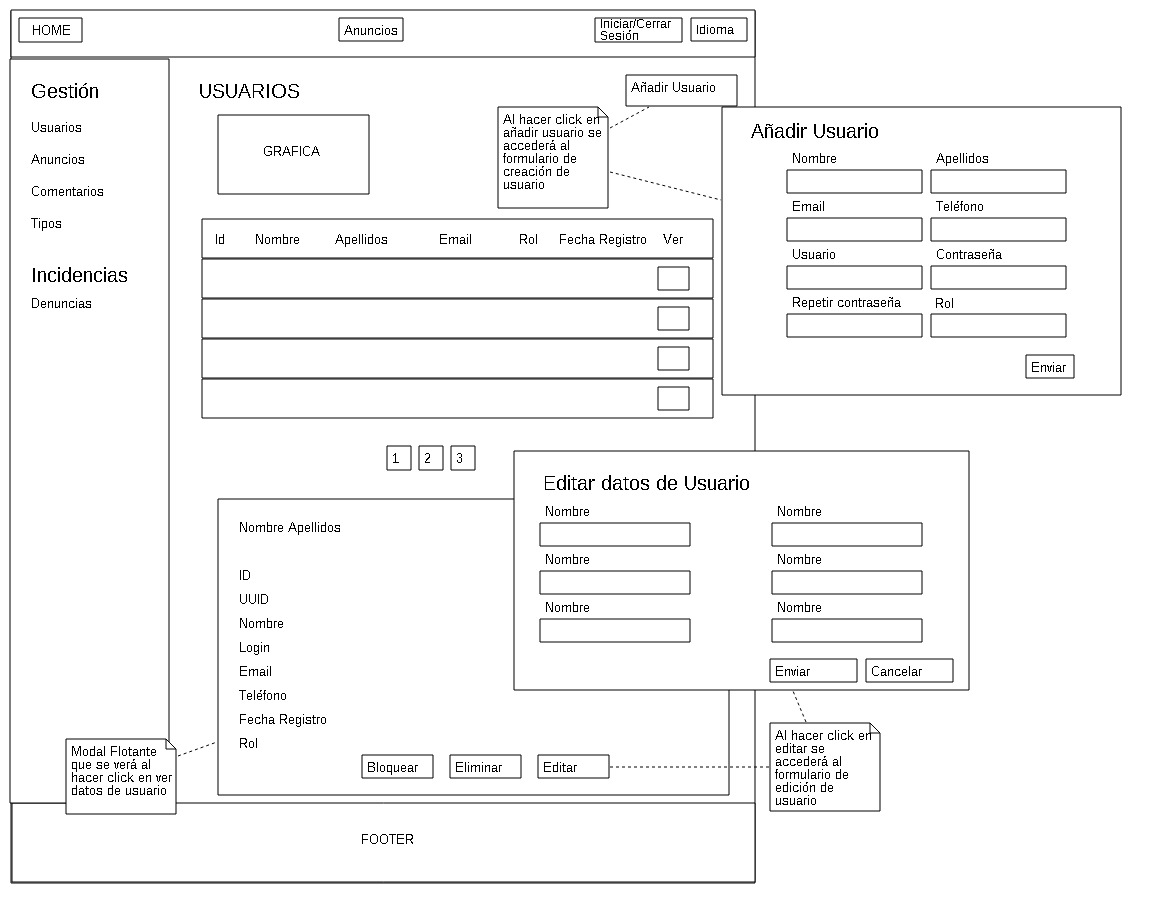
\includegraphics[width=1\textwidth]{Img/VisionAplicacion/vision_8.jpg}
\end{figure}

Primeramente, el usuario administrador ver\'{a} en su zona de administraci\'{o}n o 'dashboard' un listado de usuarios, un gr\'{a}fico con el n\'{u}mero de registros en el sistema filtrado por mes y a\~{n}o y algunos de los datos de los usuarios en una tabla debidamente paginada: \\

Id, nombre, apellidos, email, rol, fecha de registro y un bot\'{o}n que permita consultar el resto de datos asociados al usuario y acceder a m\'{a}s funcionalidades, como editar, eliminar o bloquear paginada correctamente.


\pagebreak

\subsubsection{Anuncios}
El usuario administrador podr\'{a} acceder desde su panel lateral en la zona de administraci\'{o}n a la gesti\'{o}n de los anuncios, en donde encontrar\'{a} una tabla con el id, uuid, precio, fecha registro y un bot\'{o}n que env\'{i}e a la consulta del anuncio seleccionado. Por supuesto, esta tabla estar\'{a} debidamente paginada.



\begin{figure}[h!]
\centering
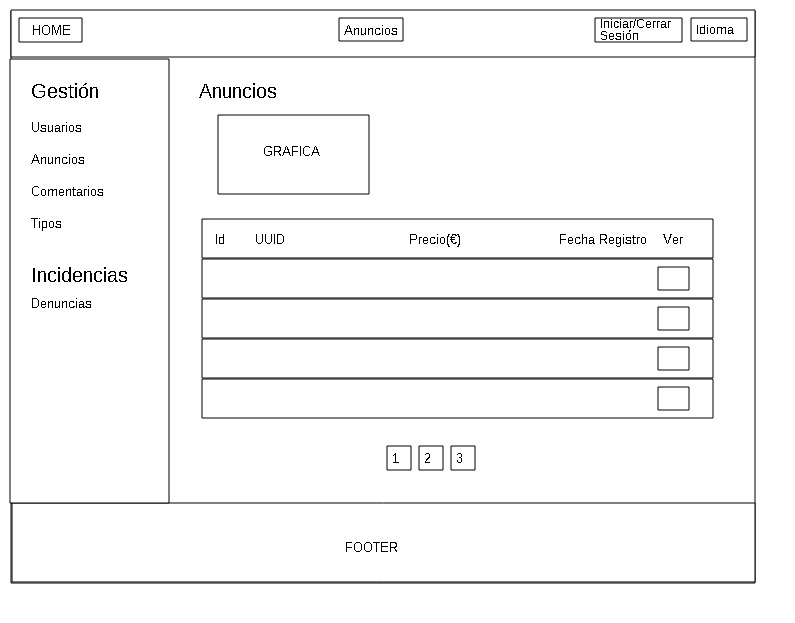
\includegraphics[width=1\textwidth]{Img/VisionAplicacion/vision_9.jpg}
\end{figure}

\pagebreak
 
\subsubsection{Comentarios}
El usuario administrador podr\'{a} acceder desde su panel lateral en la zona de administraci\'{o}n tambi\'{e}n a la gesti\'{o}n de los comentarios, donde se encontrar\'{a} una tabla con el id, anuncio, usuario, contenido, fecha registro y eliminar y un bot\'{o}n que env\'{i} a la consulta del anuncio seleccionado. Por supuesto, esta tabla tambi\'{e}n estar\'{a} debidamente paginada.

\begin{figure}[h!]
\centering
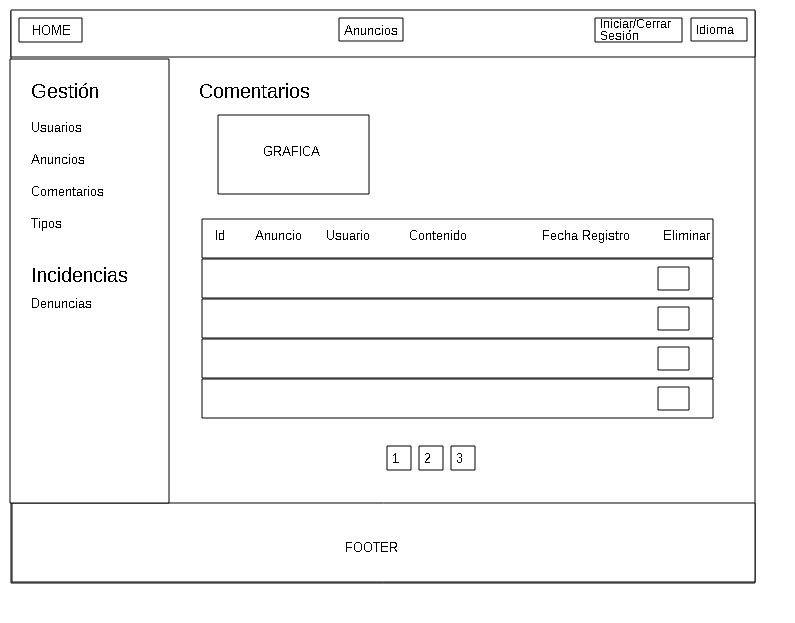
\includegraphics[width=1\textwidth]{Img/VisionAplicacion/vision_11.jpg}
\end{figure}

\pagebreak

\subsubsection{Tipos}
El usuario administrador tambi\'{e}n gestionar\'{a} los tipos de vivienda y tipos de operaciones como se puede apreciar en el siguiente mockup.\\

Ser\'{a} requisito que se gestione de forma din\'{a}mica, apareciendo modales para editar y verificar. 
\begin{figure}[h]
\centering
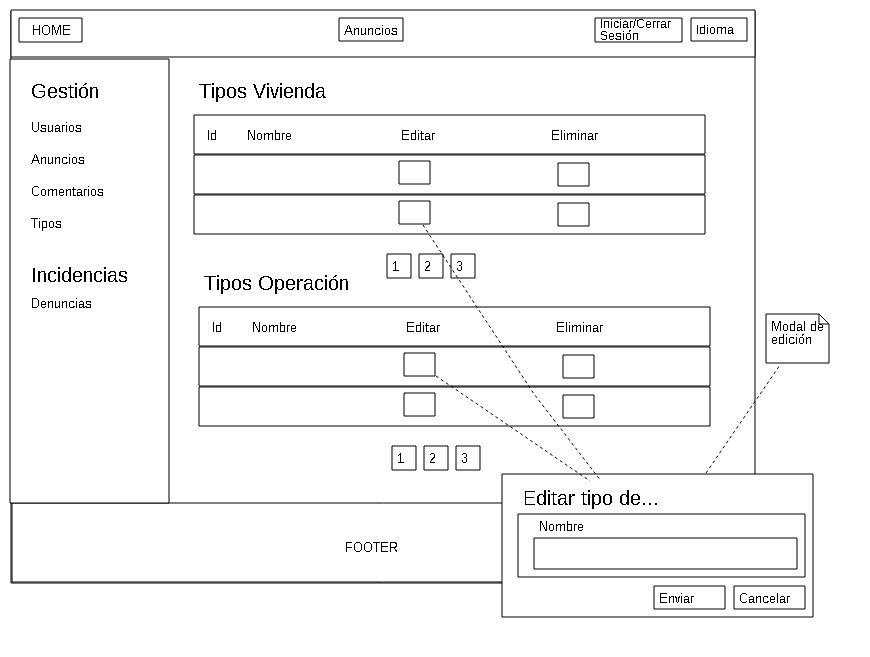
\includegraphics[width=1\textwidth]{Img/VisionAplicacion/vision_12.jpg}
\end{figure}

\pagebreak

\subsubsection{Denuncias}

Existiendo en el sistema un conjunto de usuarios, anuncios, comentarios y peticiones, es posible que exista en alg\'{u}n momento alg\'{u}n uso indebido de la aplicaci\'{o}n. Para ello, el usuario administrador recibir\'{a} y gestionar\'{a} las denuncias recibidas por otros usuarios registrados en el sistema, pudiendo aceptar o rechazar las peticiones tras haberlas consultado en los modales presentes en el siguiente mockup.

\begin{figure}[h!]
\centering
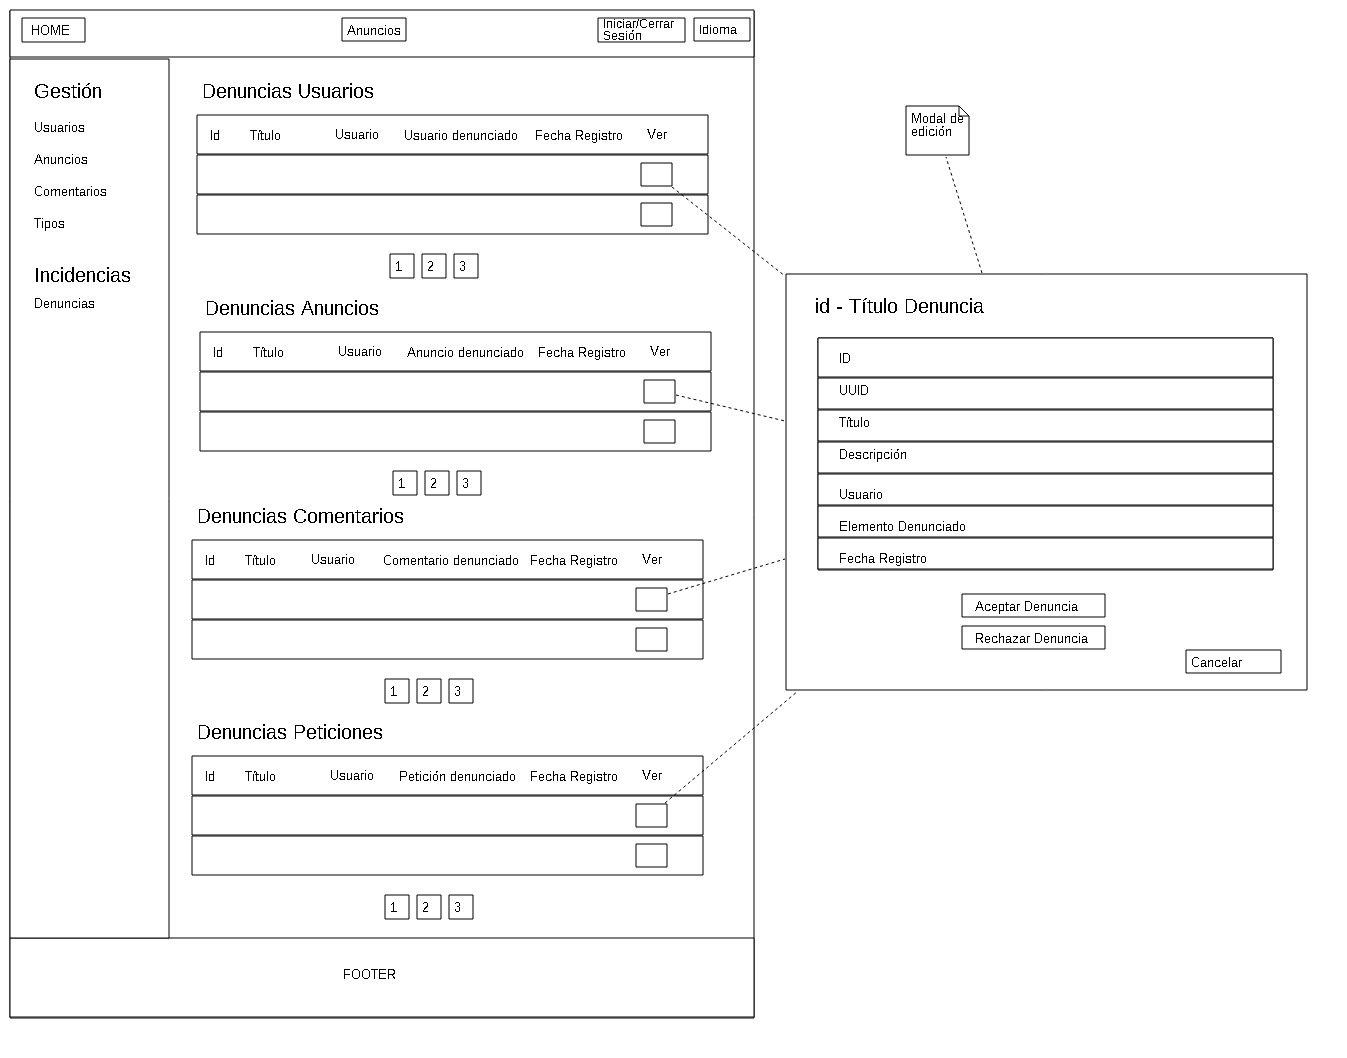
\includegraphics[width=1\textwidth]{Img/VisionAplicacion/vision_13.jpg}
\end{figure}

Los contenido de las tablas deben mostrar m\'{i}nimamente t\'{i}tulo, usuario, objeto que denuncie y fecha registro. Al ampliar deben mostrarse, al menos, uuid, t\'{i}tulo, descripci\'{o}n, usuario denunciante, referencia al objeto denunciado, contenido o similar y la fecha de registro. 

%--- Análisis ---
%--- Casos de Uso ----
\chapter{Casos de Uso}
\section{Gesti\'{o}n de Usuarios}

\begin{figure}[h]
\centering
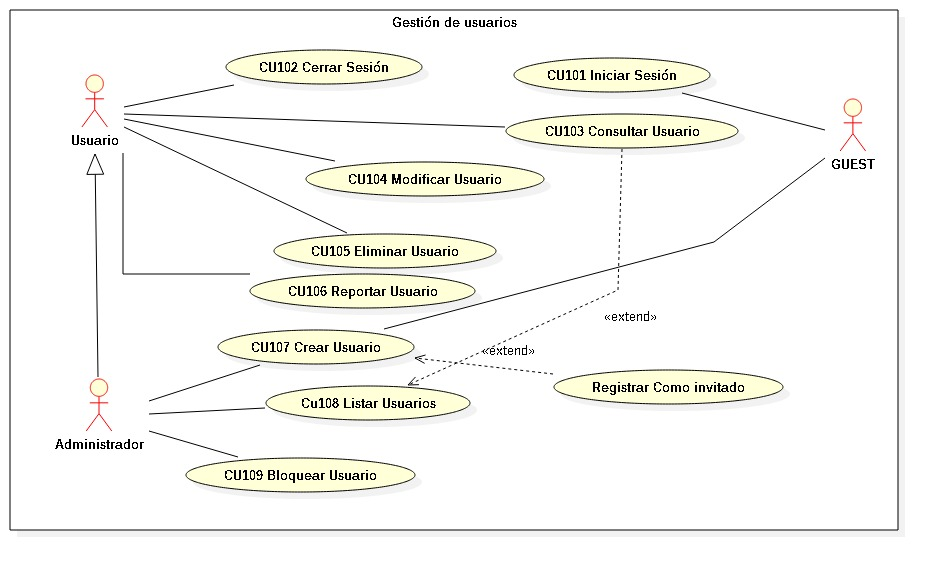
\includegraphics[width=1\textwidth]{Img/CasosDeUso/DCU01.jpg}
\caption{Diagrama de casos de uso para la gesti\'{o}n de usuarios y sesi\'{o}n.}
\label{fig:dcu}
\end{figure}

\subsection{CU101 Iniciar Sesi\'{o}n.}
\subsubsection{Descripci\'{o}n.}
El sistema identifica un usuario y guarda sus datos en la memoria para reconocerlo posteriormente.
\subsubsection{Actores.}
\begin{itemize}
\item Usuario.
\end{itemize}
\subsubsection{Poscondici\'{o}n.}
Se identific\'{o} un usuario en el sistema.
\subsubsection{Escenario Principal.}
\begin{enumerate}
\item El usuario inicia la opci\'{o}n de inicio de sesi\'{o}n.
\item El sistema solicita nombre de usuario y contrase\~{n}a.
\item El usuario introduce usuario y contrase\~{n}a.
\item El sistema valida los datos, archiva al usuario en la memoria e informa.
\item Finaliza el caso de uso.
\end{enumerate}
\subsubsection{Escenario Alternativo. L\'{i}nea 3. Datos incorrectos.}
\begin{enumerate}
\setcounter{enumi}{3}
\item El sistema informa del error.
\item Se regresa a l\'{i}nea 2.
\end{enumerate}

\subsection{CU102 Cerrar Sesi\'{o}n.}
\subsubsection{Descripci\'{o}n.}
El sistema deja de recordar al usuario que haya iniciado sesi\'{o}n.
\subsubsection{Actores.}
\begin{itemize}
\item Usuario.
\end{itemize}
\subsubsection{Precondici\'{o}n.}
\begin{itemize}
\item Usuario Logueado (CU101 Iniciar Sesi\'{o}n).
\end{itemize}
\subsubsection{Postcondici\'{o}n.}
Se dej\'{o}n de recordar al usuario en sesi\'{o}n.
\subsubsection{Escenario Principal.}
\begin{enumerate}
\item El usuario inicia la opci\'{o}n para cerrar de sesi\'{o}n.
\item El sistema deja de recordar los datos del usuario.
\end{enumerate}
Finaliza el caso de uso.
\subsection{CU103 Consultar Chat.}
\subsubsection{Descripci\'{o}n.}
El sistema permite que el usuario consulte un chat en particular de un listado de chats que se le proporciona.
\subsubsection{Actores.}
\begin{itemize}
\item Alumno.
\end{itemize}
\subsubsection{Precondici\'{o}n.}
\begin{itemize}
\item Usuario Logueado (CU101 Iniciar Sesi\'{o}n).
\end{itemize}
\subsubsection{Poscondici\'{o}n.}
Se mostr\'{o} el contenido de un chat asociado a una asignatura.
\subsubsection{Escenario Principal.}
\begin{enumerate}
\item El usuario inicia la opci\'{o}n para consultar el chat.
\item Se ejecuta el caso de uso CU104 Listar Chats.
\item El sistema muestra el contenido del chat seleccionado en el punto anterior.
\item Finaliza el caso de uso.
\end{enumerate}

\subsubsection{Escenario Alternativo. L\'{i}nea 2. El alumno cancel\'{o} la operaci\'{o}n.}
\begin{enumerate}
\setcounter{enumi}{2}
\item Finaliza el caso de uso.
\end{enumerate}

\subsubsection{Escenario Alternativo. L\'{i}nea 2. No existen datos que mostrar.}
\begin{enumerate}
\setcounter{enumi}{2}
\item El sistema informa.
\item Finaliza el caso de uso.
\end{enumerate}

\subsection{CU104 Modificar Usuario}
\subsubsection{Descripci\'{o}n}
El sistema permite que se modifiquen los datos de un usuario.
\subsubsection{Actores}
\begin{itemize}
\item Usuario.
\end{itemize}
\subsubsection{Precondici\'{o}n}
\begin{itemize}
\item Usuario Logueado (CU101 Iniciar Sesi\'{o}n).
\item Consultar usuario (CU103 Consultar usuario).
\end{itemize}
\subsubsection{Poscondici\'{o}n}
Se modificaron los datos de un usuario del sistema.
\subsubsection{Escenario Principal}
\begin{enumerate}
\item El actor acciona la opci\'{o}n para modificar los datos de un usuario.
\item El sistema solicita los datos a modificar.
\item El actor actualiza los campos y acepta.
\item El sistema valida los datos e informa.
\item Finaliza el caso de uso.
\end{enumerate}
\subsubsection{Escenario Alternativo. L\'{i}nea 3. El actor cancela la operaci\'{o}n.}
\begin{enumerate}
\setcounter{enumi}{3}
\item El sistema informa.
\item Finaliza el caso de uso.
\end{enumerate}
\subsubsection{Escenario Alternativo. L\'{i}nea 4. Datos inv\'{a}lidos.}
\begin{enumerate}
\setcounter{enumi}{4}
\item El sistema informa.
\item Se regresa a l\'{i}nea 2.
\end{enumerate}
\subsubsection{Escenario Alternativo. L\'{i}nea 4. Datos en blanco.}
\begin{enumerate}
\setcounter{enumi}{4}
\item No se actualizar\'{a}n los datos en blanco.
\item Finaliza el caso de uso.
\end{enumerate}
\subsection{CU105 Eliminar Usuario}
\subsubsection{Descripci\'{o}n}
El sistema permite que elimine un usuario.
\subsubsection{Actores}
\begin{itemize}
\item Administrador.
\end{itemize}
\subsubsection{Precondici\'{o}n}
\begin{itemize}
\item Usuario Logueado (CU101 Iniciar Sesi\'{o}n).
\item Consultar Usuario (CU103 Consultar Usuario)
\end{itemize}
\subsubsection{Postcondici\'{o}n}
Se elimin\'{o} un usuario del sistema.
\subsubsection{Escenario Principal}
\begin{enumerate}
\item El actor acciona la opci\'{o}n para eliminar al usuario.
\item El sistema solicita confirmaci\'{o}n.
\item El administrador confirma.
\item El sistema informa.
\end{enumerate}
Finaliza el caso de uso.
\subsubsection{Escenario Alternativo. L\'{i}nea 2. El actor cancela la operaci\'{o}n.}
\begin{enumerate}
\setcounter{enumi}{2}
\item El sistema informa.
\end{enumerate}
Finaliza el caso de uso.

\subsection{CU106 Consultar Privado.}
\subsubsection{Descripci\'{o}n.}
El sistema permite que el usuario consulte un privado en particular de un listado de chats privados que se le proporciona.
\subsubsection{Actores.}
\begin{itemize}
\item Delegado.
\item Profesor.
\end{itemize}
\subsubsection{Precondici\'{o}n.}
\begin{itemize}
\item Usuario Logueado (CU101 Iniciar Sesi\'{o}n).
\end{itemize}
\subsubsection{Poscondici\'{o}n.}
Se mostr\'{o} el contenido de un chat asociado a una asignatura.
\subsubsection{Escenario Principal.}
\begin{enumerate}
\item El usuario inicia la opci\'{o}n para consultar el mensaje privado.
\item Se ejecuta el caso de uso CU107 Listar Privados.
\item El sistema muestra el contenido del chat de mensajes privados seleccionado en el punto anterior.
\item Finaliza el caso de uso.
\end{enumerate}

\subsubsection{Escenario Alternativo. L\'{i}nea 2. El alumno cancel\'{o} la operaci\'{o}n.}
\begin{enumerate}
\setcounter{enumi}{2}
\item Finaliza el caso de uso.
\end{enumerate}

\subsubsection{Escenario Alternativo. L\'{i}nea 2. No existen datos que mostrar.}
\begin{enumerate}
\setcounter{enumi}{2}
\item El sistema informa.
\item Finaliza el caso de uso.
\end{enumerate}

\subsection{CU107 Crear Usuario}
\subsubsection{Descripci\'{o}n}
El sistema permite que se de de alta un usuario nuevo.
\subsubsection{Actores}
\begin{itemize}
\item Administrador.
\item GUEST.
\end{itemize}
\subsubsection{Precondici\'{o}n}
\begin{itemize}
\item El usuario es Administrador o no est\'{a} registrado en el sistema (Registro)
\end{itemize}
\subsubsection{Postcondici\'{o}n}
Se dio de alta un usuario nuevo en el sistema.
\subsubsection{Escenario Principal}
\begin{enumerate}
\item El actor acciona la opci\'{o}n para dar de alta un usuario.
\item El sistema solicita datos del usuario.
\item El actor introduce nombre, apellidos, email, tel\'{e}fono, password y acepta.
\item El sistema valida los datos e informa.
\end{enumerate}
Finaliza el caso de uso.
\subsubsection{Escenario Alternativo. L\'{i}nea 4. Datos incorrectos o usuario ya existente.}
\begin{enumerate}
\setcounter{enumi}{4}
\item El sistema informa.
\item Se vuelve al paso 2.
\end{enumerate}
\subsubsection{Escenario Alternativo. L\'{i}nea 4. Datos en blanco.}
\begin{enumerate}
\setcounter{enumi}{4}
\item El sistema informa.
\item Se vuelve al paso 2.
\end{enumerate}
\subsubsection{Escenario Alternativo. L\'{i}nea 3. El actor cancela la operaci\'{o}n.}
Finaliza el caso de uso.

\subsection{CU108 Listar Usuarios}
\subsubsection{Descripci\'{o}n}
El sistema permite que se seleccione un usuario de un listado mostrado por pantalla.
\subsubsection{Actores}
\begin{itemize}
\item Administrador.
\end{itemize}
\subsubsection{Precondici\'{o}n}
\begin{itemize}
\item Usuario Logueado (CU101 Iniciar Sesi\'{o}n).
\end{itemize}
\subsubsection{Postcondici\'{o}n}
Se mostr\'{o} un listado de usuarios del sistema.
\subsubsection{Escenario Principal}
\begin{enumerate}
\item El actor selecciona la opci\'{o}n para listar usuarios del sistema.
\item El sistema muestra un listado de usuarios paginado correctamente.
\end{enumerate}
Finaliza el caso de uso.
\subsubsection{Escenario Alternativo. L\'{i}nea 1. No existen usuarios a mostrar.}
\begin{enumerate}
\setcounter{enumi}{1}
\item El sistema informa.
\end{enumerate}
Finaliza el caso de uso.


%--- Interfaz ---
%\newpage{\pagestyle{empty}\cleardoublepage}
\newpage
\vspace*{\fill}
    \begin{center}
      \thispagestyle{empty} \vspace*{0cm} \textbf{\huge
Dise\~{n}o}
    \end{center}
    \vspace*{\fill}
\newpage{\pagestyle{empty}\cleardoublepage}
\chapter{Interfaz}
\subsubsection{Men\'{u} Principal}
\begin{itemize}
	\item[1.] Alquilar.
	\item[2.] Devolver.
	\item[3.] Consultar Alquiler.
	\item[4.] Gestionar Clientes.
	\begin{enumerate}
		\item[1.] Alta Cliente
		\item[2.] Consulta Cliente
		\begin{enumerate}
			\item[1.] Modificaci\'{o}n Cliente.
			\item[2.] Baja Cliente.
			\item[0.] Volver.
		\end{enumerate}
		\item[0.] Volver
	\end{enumerate}
	\item[5.] Gestionar M\'{a}quinas.
	\begin{enumerate}
		\item[1.] Alta Modelo
		\item[2.] Consulta modelo
		\begin{enumerate}
			\item[1.] Modificaci\'{o}n Modelo.
			\item[2.] Alta Maquinaria.
			\item[0.] Volver.
		\end{enumerate}
		\item[5.] Consulta Maquinaria
		\item[0.] Volver
	\end{enumerate}
	\item[6.] Listar Morosos
	\item[0.] Salir
\end{itemize}
%--- Diagramas de Secuencia ---
%\include{DiagramaSecuencia/Clientes}

%--- Diagrama de Clase ---
%\include{DiagramaClase/DC}

%--- Test y Datos Iniciales ---
%\newpage{\pagestyle{empty}\cleardoublepage}
\chapter{Test}

\section{Descripci\'{o}n de las pruebas realizadas}

La implementaci\'{o}n de testeo ha sido llevada a cabo con la herramienta que nos proporciona el IDE Netbeans, 'JUnit'.\\

Para esta aplicaci\'{o}n se ha realizado un testeo b\'{a}sico, contemplando flujos b\'{a}sicos y/o alternativos en cada uno de los m\'{e}todos p\'{u}blicos de la clase controlador, los diferentes modelos y la clase repositorio que contiene los datos del sistema.\\

Habiendo llegado al acuerdo anteriormente comentado con el cliente, se ha contemplado un 100\% de los m\'{e}todos a testear, o bien en su caso del flujo normal o en su caso de flujo alternativo.\\


\section{Datos de Prueba}

\subsubsection{Clientes}
\begin{figure}[h]
\begin{center}
\begin{tabular}{l*{4}{l}l}
Dni & Nombre & Direcci\'{o}n & Tel\'{e}fono \\
\hline
123456 & Alquien & Su Casa & 123456   \\
112112 & Paco & Piso 1 & 231245  \\
123123 & Pepe & S\'{o}tano 1 & 213123 \\
\end{tabular}
\end{center}
\end{figure}
\subsubsection{Modelos}
\begin{figure}[h]
\begin{center}
\begin{tabular}{l*{4}{l}l}
Nombre & Descripci\'{o}n & Stock & Precio \\
\hline
M1 & Descripcion M1 & 1 & 10   \\
M2 & Descripcion M2 & 2 & 15  \\
\end{tabular}
\end{center}
\end{figure}
\subsubsection{Maquinaria}
\begin{figure}[h]
\begin{center}
\begin{tabular}{l*{3}{l}l}
Id & Modelo & Estado \\
\hline
1 & M1 & LIBRE  \\
2 & M2 & LIBRE  \\
3 & M1 & ALQUILADA  \\
\end{tabular}
\end{center}
\end{figure}

\subsubsection{Alquileres}
\begin{figure}[h]
\begin{center}
\begin{tabular}{l*{7}{l}l}
Id & Cliente & Maquinaria & Dias & Estado & Subtotal & FechaHora\\
\hline
1 & 123456 & 3 & 2 & PENDIENTE & 20 & Actual  \\
\end{tabular}
\end{center}
\end{figure}

%\newpage{\pagestyle{empty}\cleardoublepage}


%\begin{appendix}
\chapter{Anexo: Nombrar el anexo A de acuerdo con su contenido}\label{AnexoA}
Los Anexos son documentos o elementos que complementan el cuerpo de la tesis o trabajo de investigaci\'{o}n y que se relacionan, directa o indirectamente, con la investigaci\'{o}n, tales como acetatos, cd, normas, etc.\\

\chapter{Anexo: Nombrar el anexo B de acuerdo con su contenido}
A final del documento es opcional incluir \'{\i}ndices o glosarios. \'{E}stos son listas detalladas y especializadas de los t\'{e}rminos, nombres, autores, temas, etc., que aparecen en el mismo. Sirven para facilitar su localizaci\'{o}n en el texto. Los \'{\i}ndices pueden ser alfab\'{e}ticos, cronol\'{o}gicos, num\'{e}ricos, anal\'{\i}ticos, entre otros. Luego de cada palabra, t\'{e}rmino, etc., se pone coma y el n\'{u}mero de la p\'{a}gina donde aparece esta informaci\'{o}n.\\

\chapter{Anexo: Nombrar el anexo C de acuerdo con su contenido}
MANEJO DE LA BIBLIOGRAF\'{I}A: la bibliograf\'{\i}a es la relaci\'{o}n de las fuentes documentales consultadas por el investigador para sustentar sus trabajos. Su inclusi\'{o}n es obligatoria en todo trabajo de investigaci\'{o}n. Cada referencia bibliogr\'{a}fica se inicia contra el margen izquierdo.\\

La NTC 5613 establece los requisitos para la presentaci\'{o}n de referencias bibliogr\'{a}ficas citas y notas de pie de p\'{a}gina. Sin embargo, se tiene la libertad de usar cualquier norma bibliogr\'{a}fica de acuerdo con lo acostumbrado por cada disciplina del conocimiento. En esta medida es necesario que la norma seleccionada se aplique con rigurosidad.\\

Es necesario tener en cuenta que la norma ISO 690:1987 (en Espa\~{n}a, UNE 50-104-94) es el marco internacional que da las pautas m\'{\i}nimas para las citas bibliogr\'{a}ficas de documentos impresos y publicados. A continuaci\'{o}n se lista algunas instituciones que brindan par\'{a}metros para el manejo de las referencias bibliogr\'{a}ficas:\\

\begin{center}
\centering%
\begin{tabular}{|p {7.5 cm}|p {7.5 cm}|}\hline
\arr{Instituci\'{o}n}&Disciplina de aplicaci\'{o}n\\\hline%
Modern Language Association (MLA)&Literatura, artes y humanidades\\\hline%
American Psychological Association (APA)&Ambito de la salud (psicolog\'{\i}a, medicina) y en general en todas las ciencias sociales\\\hline
Universidad de Chicago/Turabian &Periodismo, historia y humanidades.\\\hline
AMA (Asociaci\'{o}n M\'{e}dica de los Estados Unidos)&Ambito de la salud (psicolog\'{\i}a, medicina)\\\hline
Vancouver &Todas las disciplinas\\\hline
Council of Science Editors (CSE)&En la actualidad abarca diversas ciencias\\\hline
National Library of Medicine (NLM) (Biblioteca Nacional de Medicina)&En el \'{a}mbito m\'{e}dico y, por extensi\'{o}n, en ciencias.\\\hline
Harvard System of Referencing Guide &Todas las disciplinas\\\hline
JabRef y KBibTeX &Todas las disciplinas\\\hline
\end{tabular}
\end{center}

Para incluir las referencias dentro del texto y realizar lista de la bibliograf\'{\i}a en la respectiva secci\'{o}n, puede utilizar las herramientas que Latex suministra o, revisar el instructivo desarrollado por el Sistema de Bibliotecas de la Universidad Nacional de Colombia\footnote{Ver: www.sinab.unal.edu.co}, disponible en la secci\'{o}n "Servicios", opci\'{o}n "Tr\'{a}mites" y enlace "Entrega de tesis".

\end{appendix}
%\addcontentsline{toc}{chapter}{\numberline{}Bibliograf\'{\i}a}
%\nocite{alphagalileo,thesai,berkeleyAll,cscmu}
%\bibliographystyle{ieeetr}
%\bibliography{BibliMSc} 
\end{document}

